\section {Arquivador de variáveis EPICS}
%\subsection{Introdução}

\begin{frame}
\frametitle {Arquivador de variáveis EPICS}
\framesubtitle{Introdução} 

\begin{itemize}
  \item \textit{Management}: gerência da \textit{appliance}.
  \item \textit{Engine}: integração entre os módulos.
  \item \textit{Data Retrieval}: recuperar os dados das \textit{PVs} arquivadas.
  \item \textit{ETL}: extrair os dados das unidades de armazenamento.

\end{itemize}

\begin{figure}[h]

    \centering
    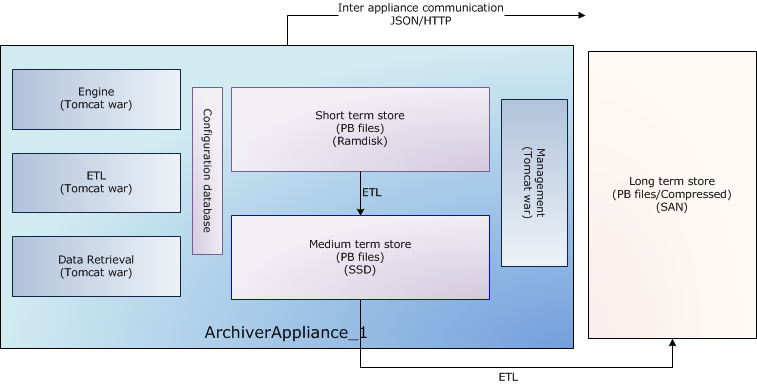
\includegraphics[scale=0.3]{image/applarch}
    \caption {Modo de funcionamento de uma \textit{appliance}.}
    \label{fig:epics_archiver}
\end{figure}

\end{frame}

%\subsection{Modificações}

\begin{frame}
\frametitle {Arquivador de variáveis EPICS}
\framesubtitle{Modificações}

\begin{itemize}
  \item Interfaces de \textit{login}:
  \begin{itemize}
    \item Problema: qualquer pessoa logada pode inserir ou remover variáveis do
    sistema.
    \item Instalação de um servidor LDAP: no futuro, integrar com o servidor
    LDAP do CNPEM.
    \item Módulo PHP: realiza a comunicação entre servidor LDAP e usuário e
    retorna se a autenticação foi bem sucedida ou não.
    \item Em caso de sucesso, outra requisição POST é enviada ao módulo de
    \textit{management}.
    \item Módulo de \textit{management}: inicia uma nova sessão para o usuário.
  \end{itemize}
  \item Modificações nos arquivos \texttt{.css}.
\end{itemize}

\end{frame}

%\subsection{Resultados}

\begin{frame}
\frametitle {Arquivador de variáveis EPICS}
\framesubtitle{Resultados}

\begin{figure}[h]

\centering
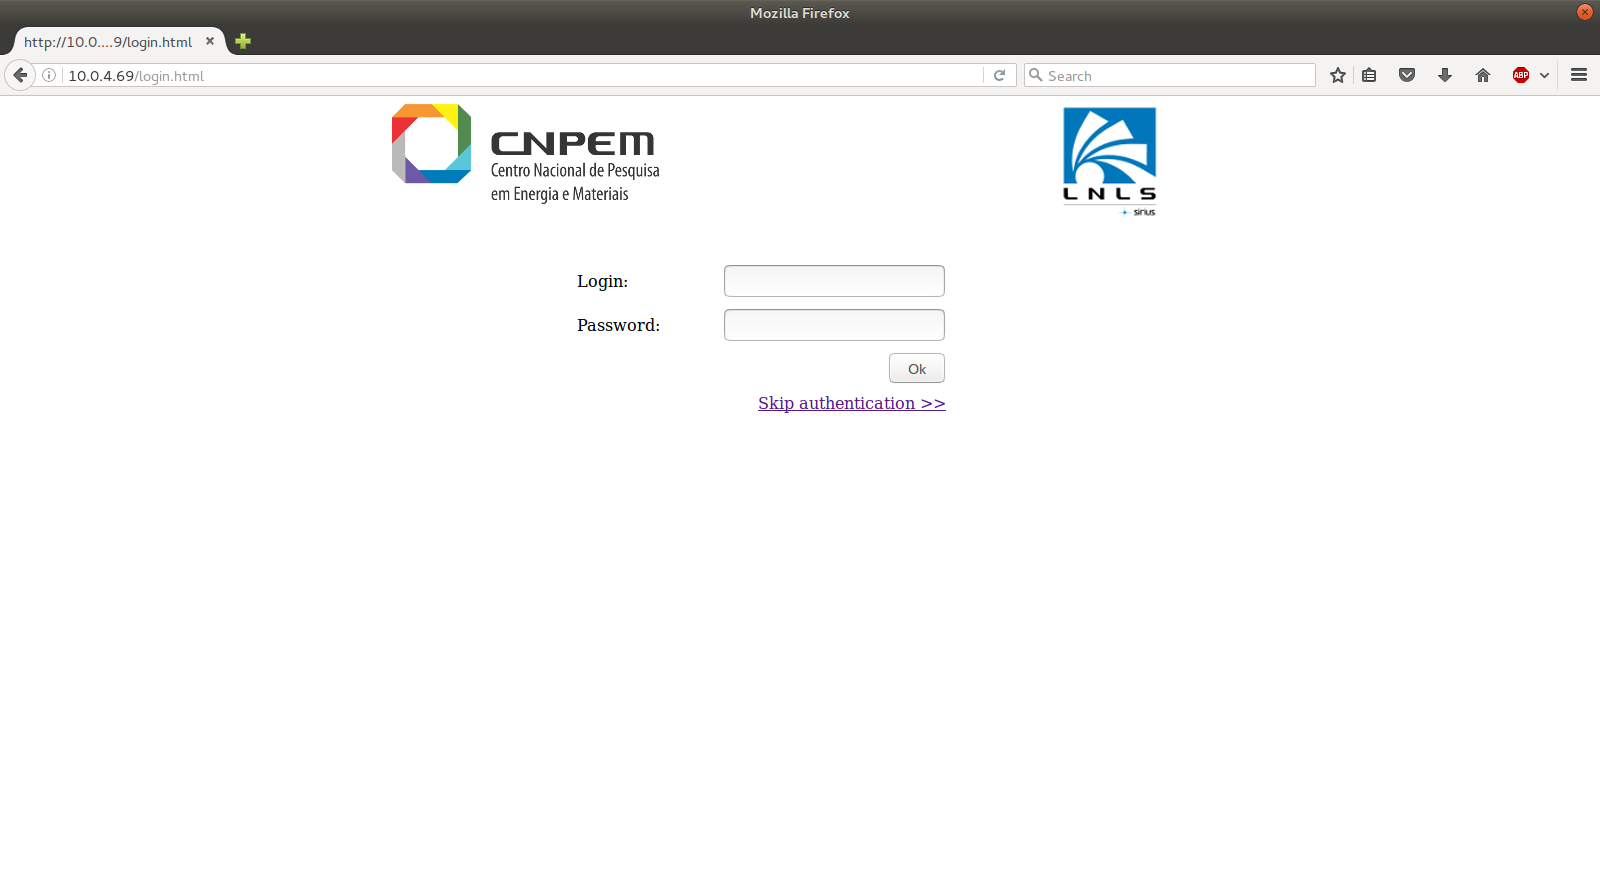
\includegraphics[width=0.93\textwidth]{image/login}
\caption {tela de \textit{login} para o \textit{archiver} instalado no OPR23.}
\label{fig:login}
\end{figure}

\end{frame}

\begin{frame}
\frametitle {Arquivador de variáveis EPICS}
\framesubtitle{Resultados}

\begin{figure}[h]

\centering
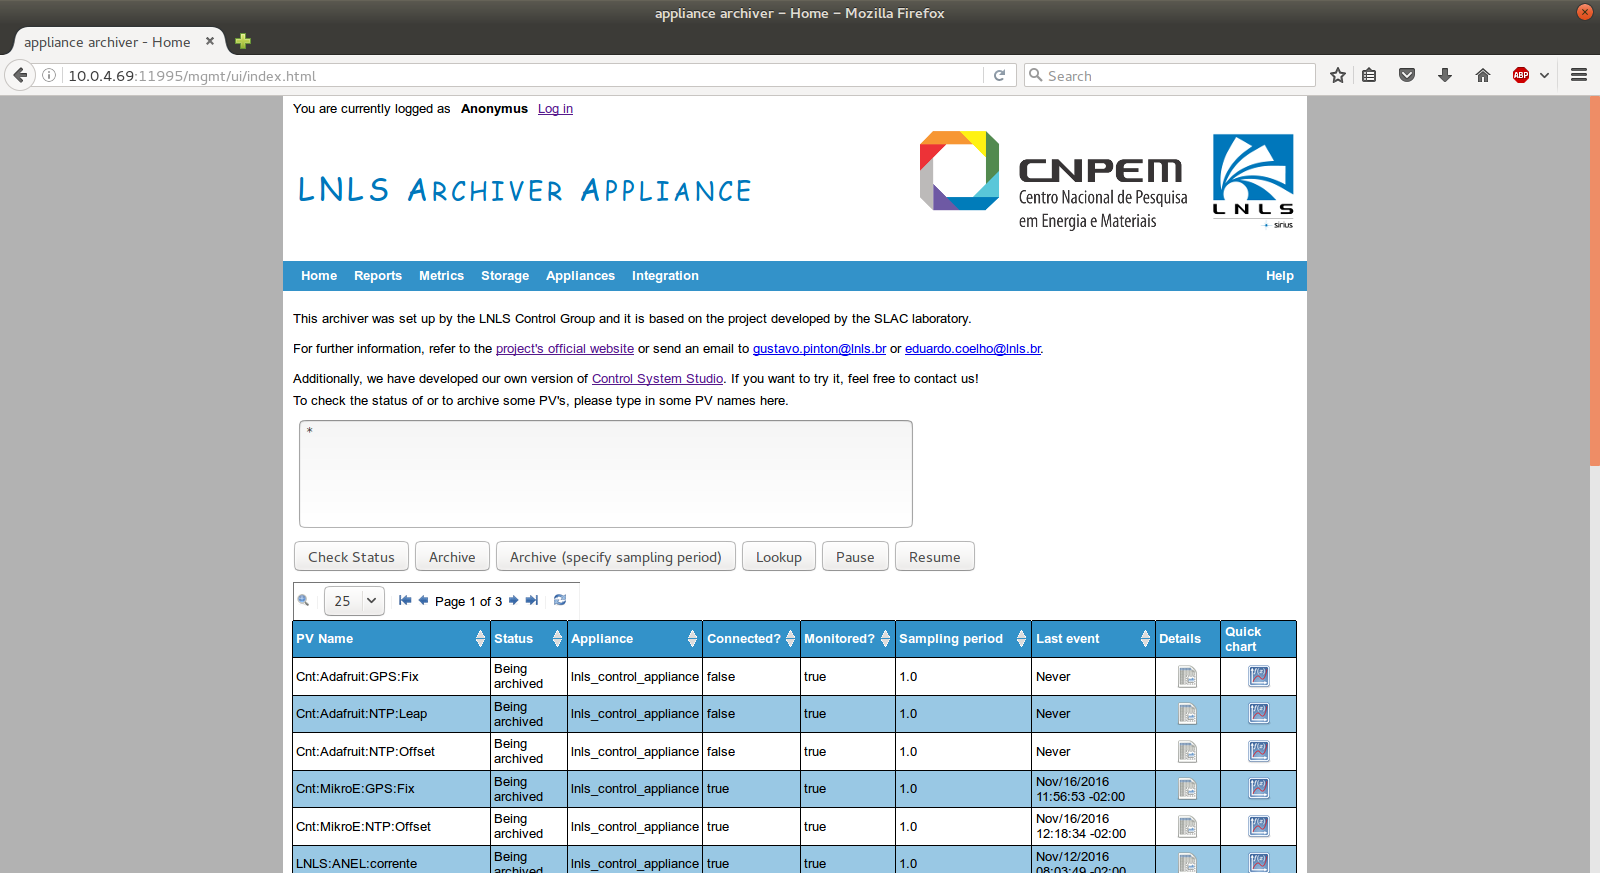
\includegraphics[width=0.93\textwidth]{image/archiver}
\caption {\textit{Archiver} instalado no OPR23.}
\label{fig:archiver}
\end{figure}

\end{frame}